\documentclass[conference]{IEEEtran}


  	\usepackage[pdftex]{graphicx}
  	\graphicspath{{./assets}{../jpeg/}}
	\DeclareGraphicsExtensions{.pdf,.jpeg,.png}

	\usepackage[cmex10]{amsmath}
	\usepackage{mathabx}
	\usepackage{algorithmic}
	\usepackage{array}
	\usepackage{mdwmath}
	\usepackage{mdwtab}
	\usepackage{eqparbox}
	\usepackage{url}
	\hyphenation{op-tical net-works semi-conduc-tor}


\begin{document}

\title{\LARGE Modeling of Trap Induced Dispersion of Large Signal Dynamic Characteristics of GaN HEMTs}

% \author{\authorblockN{Leave Author List blank for your IMS2013 Summary (initial) submission.\\ IMS2013 will be rigorously enforcing the new double-blind reviewing requirements.}
% \authorblockA{\IEEEauthorrefmark{1}Leave Affiliation List blank for your Summary (initial) submission}}

\author{\IEEEauthorblockN{O. Jardel\IEEEauthorrefmark{1}, S. Laurent\IEEEauthorrefmark{2}, T. Reveyrand\IEEEauthorrefmark{2}, R. Qu\'{e}r\'{e}\IEEEauthorrefmark{2}, P. Nakkala\IEEEauthorrefmark{2}, A. Martin\IEEEauthorrefmark{2}\\ S. Piotrowicz\IEEEauthorrefmark{1}, M. Campovecchio\IEEEauthorrefmark{2}, S.L. Delage\IEEEauthorrefmark{1} }
\IEEEauthorblockA{\IEEEauthorrefmark{1}III-V Lab, route de Nozay, 91461 Marcoussis Cedex, France}
\IEEEauthorblockA{\IEEEauthorrefmark{2}XLIM, 7 rue Jules Valles, 19100 Brive-la-gaillarde, France\\olivier.jardel@3-5lab.fr}}

\maketitle

\begin{abstract}
    We propose here a non-linear GaN HEMT model for CAD including a trapping effects description consistent with both small-signal and large-signal operating modes. It takes into account the dynamics of the traps and then allows to accurately model the modulated large signal characteristics that are encountered in telecommunication and radar signals. This model is elaborated through low-frequency S-parameter measurements complementary to more classical pulsed-IV characterizations. A 8x75$\mu$m AlInN/GaN HEMT model was designed and particularly validated in large-signal pulsed RF operation. It is also shown that thermal and trapping effects have opposite effects on the output conductance, thus opening the way for separate characterizations of the two effects.
\end{abstract}

\IEEEoverridecommandlockouts
\begin{IEEEkeywords}
    Trappings effects, thermal effects, low frequency S-parameters, CAD non-linear model, RF pulsed operation.
\end{IEEEkeywords}

\IEEEpeerreviewmaketitle


% ===================
% # I. Introduction #
% ===================

\section{Introduction}
Gallium Nitride (GaN) High Electron Mobility Transistors (HEMT) on SiC are now recognized as good candidates for the development of a number of RF applications and notably Power Amplifiers (PA) for telecommunications and radars, due to their high breakdown voltage, their high cut-off frequency as well as their high temperature capabilities. However they are still subject to parasitics effects such as thermal effects and especially trapping effects. Those trapping effects have been extensively studied using a number of techniques such as pulsed measurements, load-pull measurements as well as frequency dispersion measurements. At the same time, models have been proposed that take those effects into account \cite{5296056, Leoni2001, 5516843}, and while the effects of traps are well taken into account in CW conditions, their impacts on dynamic large signal characteristics remain difficult to understand. They manifest themselves under modulated signals such as RF pulses or telecommunications signals. Memory effects are the main consequence of those trapping effects. In this paper we propose to investigate the dynamics of those trapping effects using large signal pulsed load pull measurements as well as low frequency dispersion measurements. It will be shown that a consistent nonlinear model can be obtained that allows to describe the full dynamic behavior of GaN transistors. The paper is organized as follows: Section II describes the theoretical impact of traps on the average current obtained under pulsed load pull conditions. Section III presents the measurements performed on an AlInN/GaN 8x75$\mu m$ HEMT and the results obtained using a large signal nonlinear electrothermal model taking into account the dynamics of the traps. Finally we conclude and draw some perspectives.


% =======================================================
% # II. Impact of traps on large signal characteristics #
% =======================================================

\section{Impact of traps on large signal characteristics}
One convenient way to identify the impact of trapping effects is to monitor the average drain current of the transistor versus an increasing RF input power. It has already been reportedbegin in \cite{5296056} and \cite{5516843} that this drain current under class-AB conditions decreases as the input power increases, contradicting the expected characteristics. Clearly this behavior cannot be explained by thermal behavior as far as the channel temperature sinks when the power increases and would leads, at least for moderate powers, to an average drain current enlargement.

\begin{figure}[ht!] %!t
    \centering
    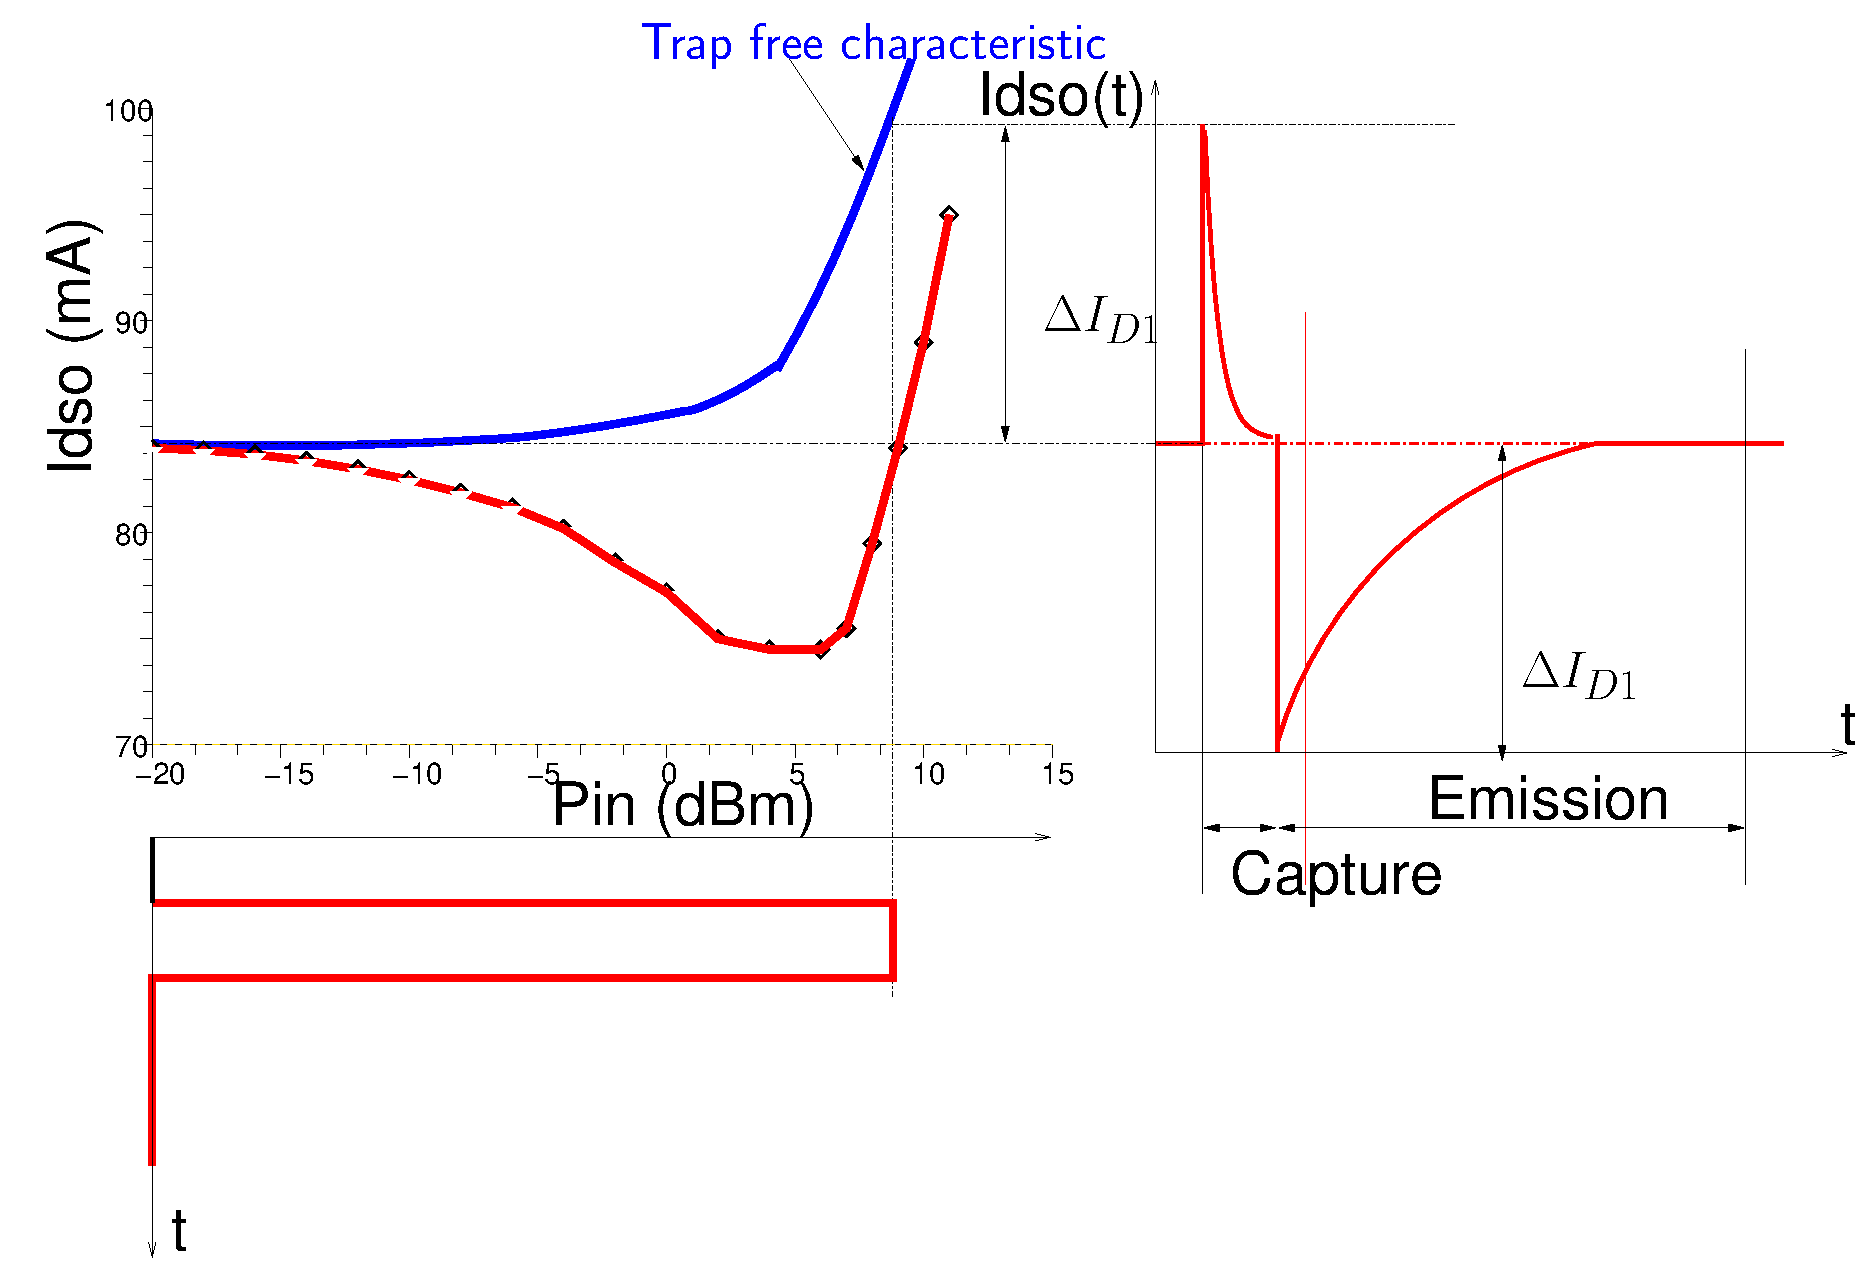
\includegraphics[width=3.5in]{Courant_2.pdf}
    \caption{Representation of the mechanism induced by traps on the average drain current.}
    \label{Courant_2}
\end{figure}

Pulsed RF measurements were performed under DC bias on  AlGaN/GaN and InAlN/GaN HEMTs of 8x75x0.25$\mu m^2$ for a large number of output loads. For all devices, we obtain the same shape of the average drain current which is shematized in Figure \ref{Courant_2}. The average current decrease is due to the trap capture, which increases alike to the gate and drain voltage excursions versus the input power for a CW measurement. Indeed, the number of ionized traps is roughly proportional to the maximum value of the drain-source voltage, because of the disymmetry of the capture and emission time constants \cite{163456}.  When the RF power is pulsed, the average drain current exhibits transients  corresponding to the capture and emission of traps. For example, if the RF input power is pulsed to 0dBm, the current decreases  within the pulse due to the capture of traps. At the end of the pulse, when the input power is switched-off, there is a discontinuity in the drain current corresponding to the amount of increase ($\Delta I_{D1}$) of the average drain current, which should have appeared in the absence of traps as shown in Figure \ref{Courant_2}. Then the captured carriers are re-emitted and the drain current recovers at its bias level. It can be seen that the emission time constant for emission remains in the ms range while the capture one is lower than 10$\mu s$.


% =============================================
% # III. Modeling and consistency validations #
% =============================================

\section{Modeling and consistency validations}

A previous large signal model including a description of the trapping effects \cite{Jardel2007b} was able to the reproduce the dynamics of the trapping effects versus the swings of the command voltages $V_{gs}$ and $V_{ds}$, i.e. by extension versus the input power and the load impedances during CW load-pull measurements. This allowed hence modeling consistently the typical shape of the average current, leading to an important improvement of the model accuracy.

For this study, a 8x75$\mu$m AlInN/GaN HEMT has been characterized and modeled. The transistor is processed on SiC substrate using 0.25$\mu$m T-Gates technology. More details on the technological process of this transistor are given in \cite{jardel2012first}.
The model takes into account thermal, gate-lag and drain-lag effects, and a special care was taken on its accuracy for CW power performances prediction at 10GHz, for a nominal bias point $V_{ds}$=15 to 25V, $I_{ds}$=250mA/mm.
Fig. \ref{LP} shows the measured CW RF power characteristics at 10.24 GHz of a transistor biased at $V_{ds}$=20V, $I_{ds}$=150mA.  It delivers, on the optimum load impedance $Z_{load}=20+j.18\Omega$ and exibit 4.8W/mm output power at 3.5dB of compression with a PAE of 46\% and an associated gain of 11.5dB.

\begin{figure}[ht!] %!t
    \centering
    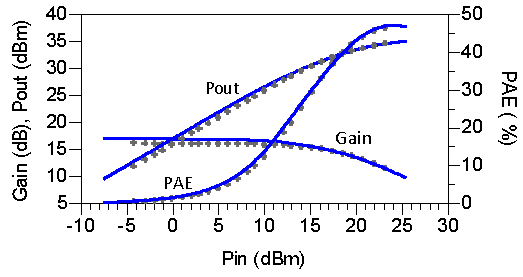
\includegraphics[width=3.5in]{FigureLP_ancien_mod.pdf}
    \caption{Measurements (grey), modeling (blue) of the CW RF performances of a 8x75$\mu$m AlInN/GaN HEMT at 10.24GHz in class AB. $Z_{loadOPT} = (20+j.18) \Omega$.}
    \label{LP}
\end{figure}

However, using this model, the transient dynamics of the average current during pulsed power RF measurements is not sufficient as was already observed in \cite{wamicon}.
Even if the output current behavior, due to capture and release of charges by traps is consistent as both processes are taken into account, the amplitude of the discontinuity of the current (named $\Delta I_{D1}$ in Figure \ref{Courant_2}), observed at the moment when the RF signal is switched off, has not enough amplitude. This can be explained by the fact that the extraction of the drain-lag contribution from pulsed-IV measurements at different quiescent bias points is a too much rough method to provide a correct traps induced current dispersion, especially around the nominal bias point, which is moreover often at low current in amplifiers. This however allows to model enough precisely the IV characteristics in the area of the IV network where the current is high and the drain voltage is close to the knee voltage, and where the traps induced current dispersion limits the RF load lines swing under RF power drive. This explains the good capability of the previous model to fit RF power characteristics despite the use of pulsed IV networks to model the lag correction terms.

We propose here to use low-frequency S-parameters measurements \cite{elrafei} instead or in addition to pulsed IV measurements, which represent a far more precise and convenient method to extract the drain-lag contribution in the transistors non-linear models. Precise because the S-parameters do not provide the current, but directly its derivative. The output conductance is expressed by $g_d=\Re \left\{Y(2,2)\right\}$. $g_d$ is very sensitive to the drain-lag trapping effects, in the frequency range of the emission time constants of these traps.

Convenient because the variations of the output conductance also provide the detrapping and thermal time constants, and give the ability to separate both effects, which induce opposite $g_d$ variations. However, traps time constants are particularly dependent on the electric fields and the temperature conditions (i.e. the measurement bias point), and these variations are not taken into account in the drain-lag model for the moment. Thus, the modeled traps time constants are fixed at the values measured with low frequency S-parameters at the nominal bias point of the application.

The amplitude of the correction term is also determined from the same measurement, at the nominal bias point, in order to get the correct dispersion level in pulsed RF case, when RF is switched off and the transistor goes back to its nominal bias point. This however highlighted an imprecision of the previous model, in which the dispersion correction term was added to the command voltage vgs. Indeed, the fit of the output conductance dispersion induced by trapping effects leaded to a too high level of dispersion at high current, i.e. where the RF signal swings during power RF operation, thus inducing too much power slump in such cases. The model has been modified in order to add this correction term to the pinch-off voltage ($v_p$) formulation and also to the parameter $I_{DSS}$ (determining the steady state current) into the current source equations. Both contributions are written in order to conserve the proportionality relationship between $v_p$ and $I_{DSS}$. It allows to get a more precise dependence of the dispersion versus the current Ids delivered by the current source.

\begin{figure}[ht!] %!t
    \centering
    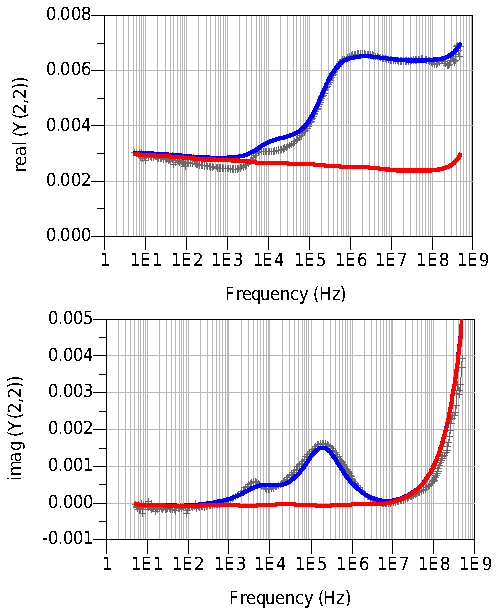
\includegraphics[width=3.0in]{Compare_S.pdf}
    \caption{$\Re\{Y_{22}\}$ and $\Im\{Y_{22}\}$. AlInN/GaN 8x75 $\mu m$ HEMT measurements at $V_{ds}=20V$, $I_{ds}=120mA$ (grey) are compared to a simple eletro-thermal model (red) and an eleectro-thermal model including activated drain-lag effects (blue)}
    \label{Compare_S}
\end{figure}

A low-frequency S-parameters comparison between measurements and simulation at $V_{ds}$=20V, $I_{ds}$=200mA/mm is presented at Figure \ref{Compare_S}. The measurements have been performed between 5Hz and 500MHz in order to capture all the variations range of the thermal and trapping effects.

We can observe two main traps having emission time constants leading to an increase of gd in the range of 2kHz-8kHz and 20kHz-1MHz, respectively. Thermal effects induce a decrease of the output conductance. The thermal model was determined from a three-dimensional finite element (3D-FE) simulation, and in order to take into account the distribution of the time constants, five RC-cells (i.e. five time constants) are necessary. However, the thermal contribution on the output conductance is quite negligible, as can be seen on the red curve that corresponds to the model with thermal effects only (trapping effects are desactivated).

The imaginary part of $Y(2,2)$ is also presented, and a good agreement between the measurements and the simulations with this non-linear electrothermal model can also be observed. One can see that this imaginary part exhibits two maxima, which correspond to two kinds of drain-lag inducing traps. Thus this kind of measurement provides a convenient way to identify various types of traps in the transistor.

\begin{figure}[ht!] %!t
    \centering
    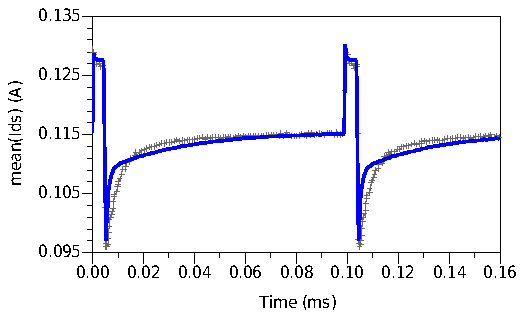
\includegraphics[width=3.0in]{Compare_pulse.pdf}
    \caption{Measurements (grey) and modeling (blue) of the average output current in pulsed RF signal operation at 10 GHz (5$\mu$s-100$\mu$s) with DC bias (20V, 115 mA). The amplitude of the transcient induced by detrapping when RF is switched off is accurately modeled.}
    \label{Compare_pulse}
\end{figure}

Figure \ref{Compare_pulse} shows a comparison between RF pulsed measurements and simulations with this model. The transistor is measured at Vds0=20V, Ids0=115mA (190mA/mm), on a load impedance $Z_{load}=\left(20+j18\right)\Omega$. The bias voltages are continuous, and the RF signal, at a frequency of 10GHz, is pulsed. Its duration is 5$\mu s$, and its period 100$\mu s$. On this example, the RF imput power equals 20dBm, corresponding approximately to 1dB of gain compression. The very large amplitude of the current discontinuity at the moment when RF is switched off leads to a transient current from 97mA to 115mA (i.e. the nominal bias point).

Envelope-transient simulations show the modeled output current, and the model enhanced capability to reproduce both the current discontinuity and the slow transient due to traps emission. The emission time constants are however not very accurate, and this can be due by the strong non-linearity of traps time constants versus bias and temperature, as explained previously.


% ==================
% # IV. CONCLUSION #
% ==================

\section{Conclusion}
This work shows the importance of an accurate modeling of trapping effects in GaN HEMTs when they are used in large signal dynamic operation. An existing version of non-linear model including trapping effects has been improved in order to give better consistency between the dispersion effects around the nominal bias point and in the high $I_{ds}$-low $V_{ds}$ area, the first determining the model accuracy when the RF is switched off during pulsed RF operation, the latter the model accuracy under CW operation, or when RF is on during RF pulsed operation.

Further work will investigate the behavior of the model under other types of dynamic RF operation like two-tone characteristics, and also on the improvement of the dispersion amplitude and detrapping time constants accuracies over the whole IV characteristics by fitting low frequency S-parameters measured at several bias points.


% ==================
% # ACKNOWLEDGMENTS #
% ==================

% use section* for acknowledgement
%\section*{Acknowledgment}
% The authors would like to thank...


% ==============
% # REFERENCES #
% ==============

\bibliographystyle{IEEEtran}
\bibliography{IEEEabrv,bibliography}

\end{document}
